\chapter[Transfer learning ++]{Transfer learning ++}
\label{chap:Transfer_learning}
\begin{chapabstract}
    This chapter highlights the superior capacities of transfer learning of the HiDeNN framework.
\end{chapabstract}

\minitoc

\section{Leveraging pre-trained model}

Because the architecture of HiDeNN is fully interpretable, the initialisation of the weights for a new (refined for instance) architecture can be done by using a previously trained architecture ( coarser one for instance).

\Rq{This is true for a new architecture with 
\begin{itemize}
    \item A refined space mesh
    \item A refined parametric mesh
    \item A different number of parameters
    \item A different number of modes
\end{itemize}}

\subsection{Training a finer space mesh}

When a new node $\ell$ is added at coordinate $\vect{x}_{\ell}$, the nodal value (the weights of the solution layer) can be initialised using the interpolation of the previously trained network as
\begin{equation}
    u_{\ell} = \vect{u}\left(\vect{x}_{\ell}\right).
\end{equation}

For a completely different mesh (refined) we can easily evaluate the coarse model on fine mesh and use the solution as initial nodal value for the fine HiDeNN. Here the finer model consist in a refined space mesh; the parametric mesh remains exactly the same.

A space refinement from $n_p = 20$ to $n_p = 60$ is investigated.
Illustrations of different initialisation strategies are given in \cref{fig:TransferSpace} where 
\begin{equation}
    \Xi = \frac{\Vert\overline{ \vect{u}_{NN}-\vect{u}_{\text{exact}}}\Vert}{\Vert\overline{ \vect{u}_{\text{exact}}}\Vert}.
\end{equation}

$\overline{\square}$ is the average of the quantity $\square$ over the samples of $E$.

\begin{figure}
    \begin{subfigure}[t]{0.5\linewidth}
        \centering
        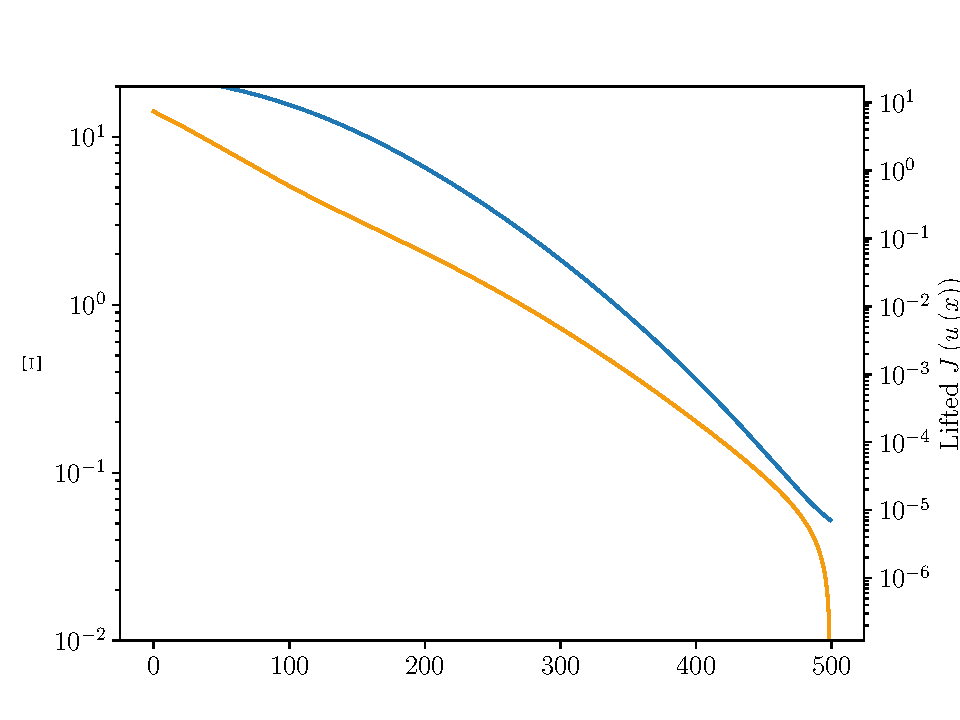
\includegraphics[width=\linewidth]{Figures/ParaError_NoInit.pdf}
        \caption{No initialisation}
    \end{subfigure}
    \begin{subfigure}[t]{0.5\linewidth}
        \centering
        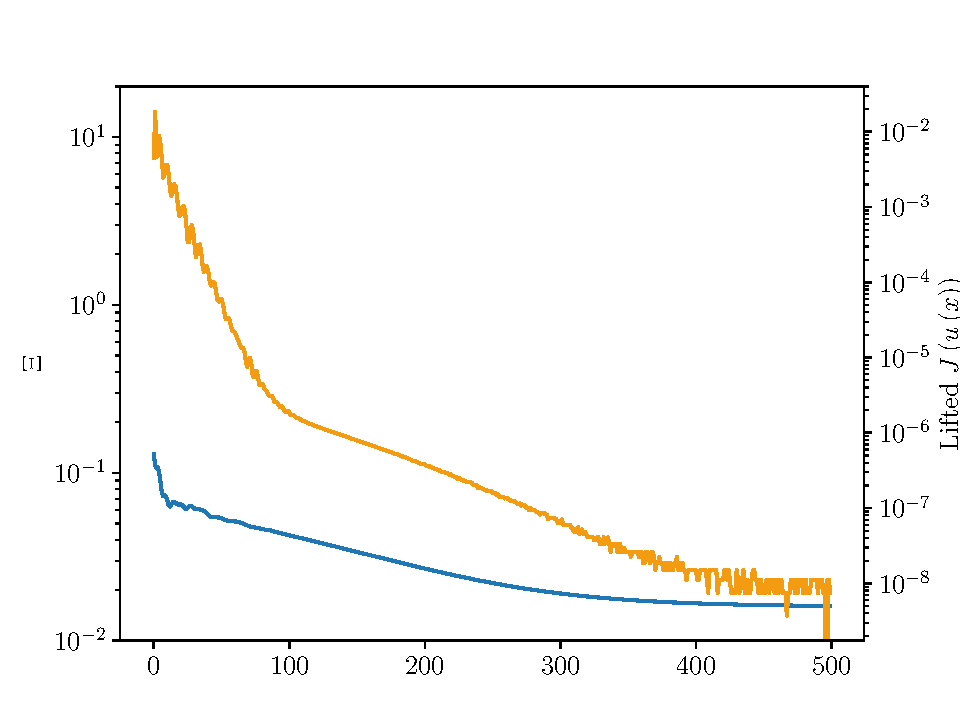
\includegraphics[width=\linewidth]{Figures/ParaError_full_initialised.pdf}
        \caption{Space and parameter modes initialised}
    \end{subfigure}
    \begin{subfigure}[t]{0.5\linewidth}
        \centering
        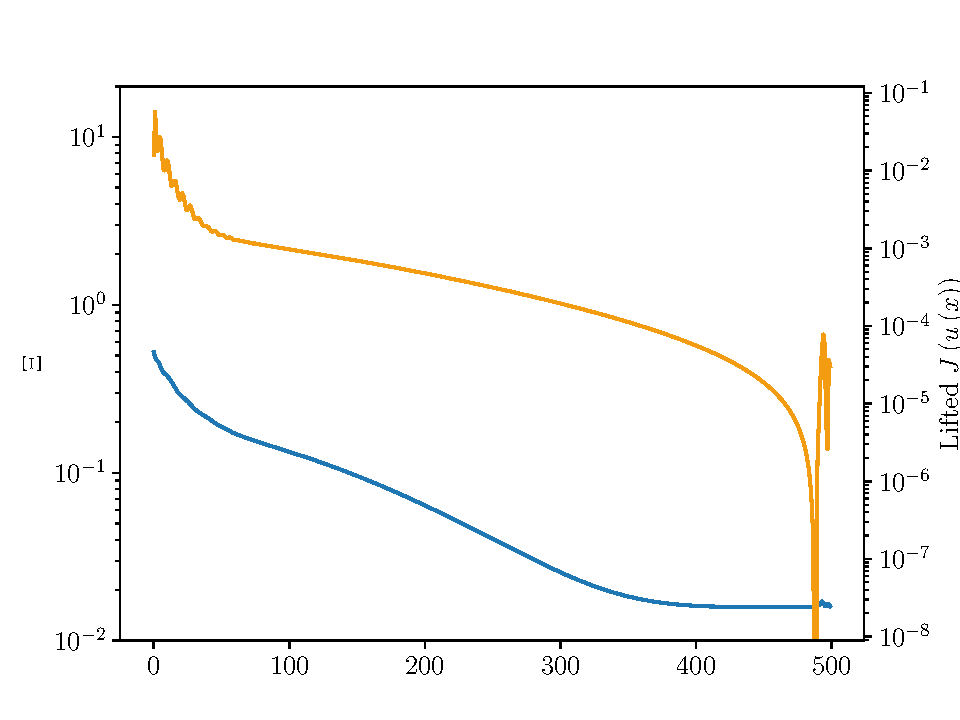
\includegraphics[width=\linewidth]{Figures/ParaError_space_initialised.pdf}
        \caption{Space mode initialised}
    \end{subfigure}
    \begin{subfigure}[t]{0.5\linewidth}
        \centering
        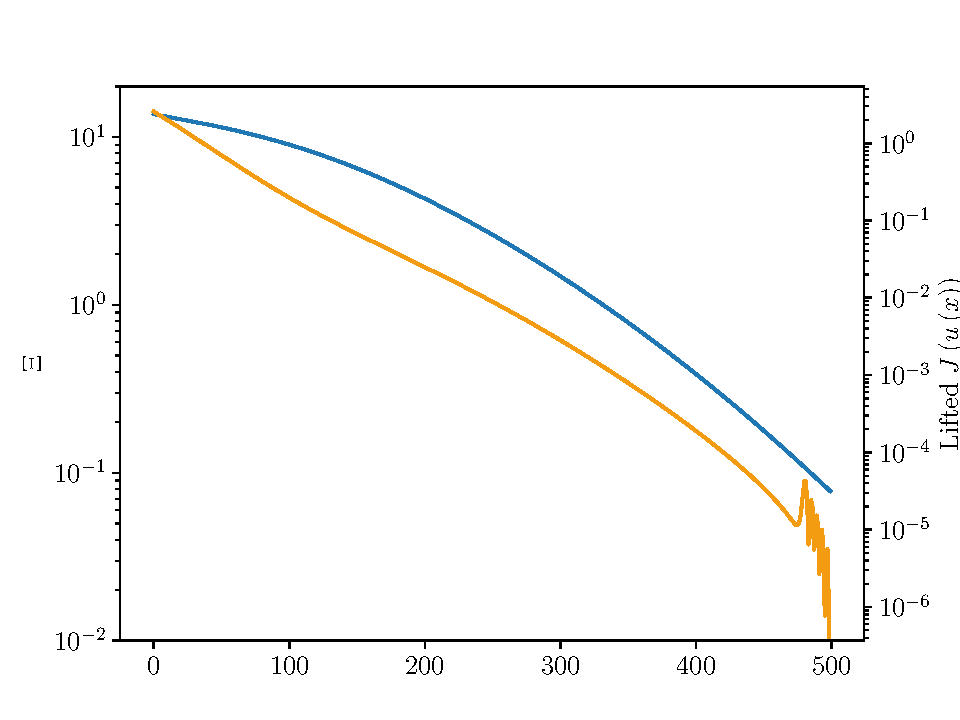
\includegraphics[width=\linewidth]{Figures/ParaError_para_initialised.pdf}
        \caption{Parameter mode initialised}
    \end{subfigure}
        \caption{Loss and $\mathcal{L}^2$ error}
    \label{fig:TransferSpace}
\end{figure}

An illustration of the use of pretrained coarse modes to quickly get a fine mode is illustrated in \cref{fig:InitialisationModes_Coarse}.

\begin{figure}
    \begin{subfigure}[t]{0.5\linewidth}
        \centering
        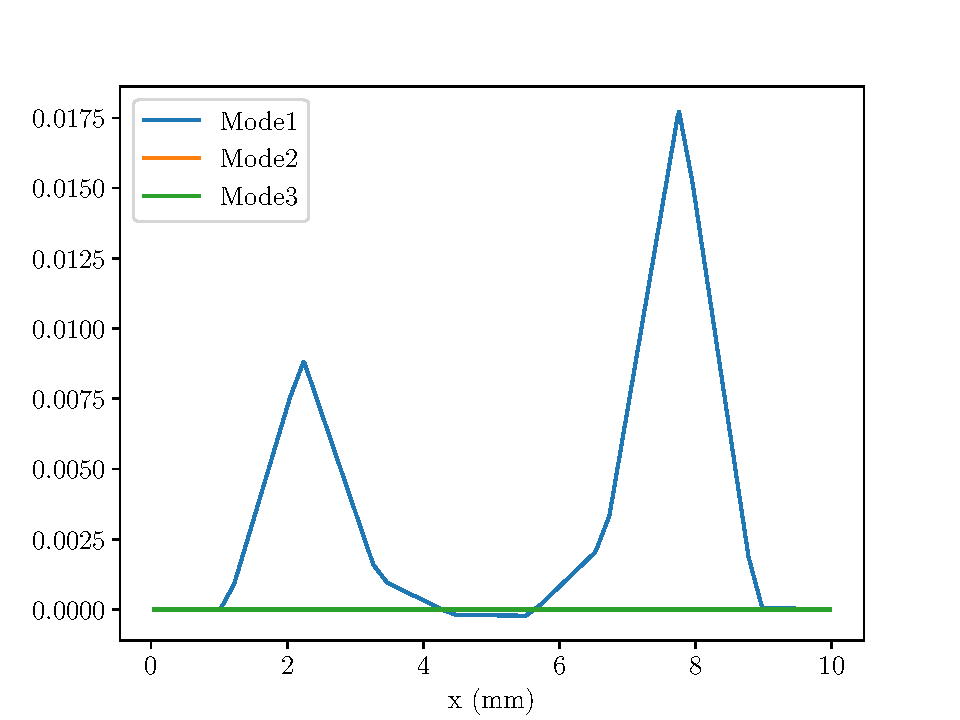
\includegraphics[width=\linewidth]{Figures/Pre_trained_Space_modes3.pdf}
        \caption{Pre-trained space mode initialisation on $1$ mode \& $n_p=10$}
    \end{subfigure}
    \begin{subfigure}[t]{0.5\linewidth}
        \centering
        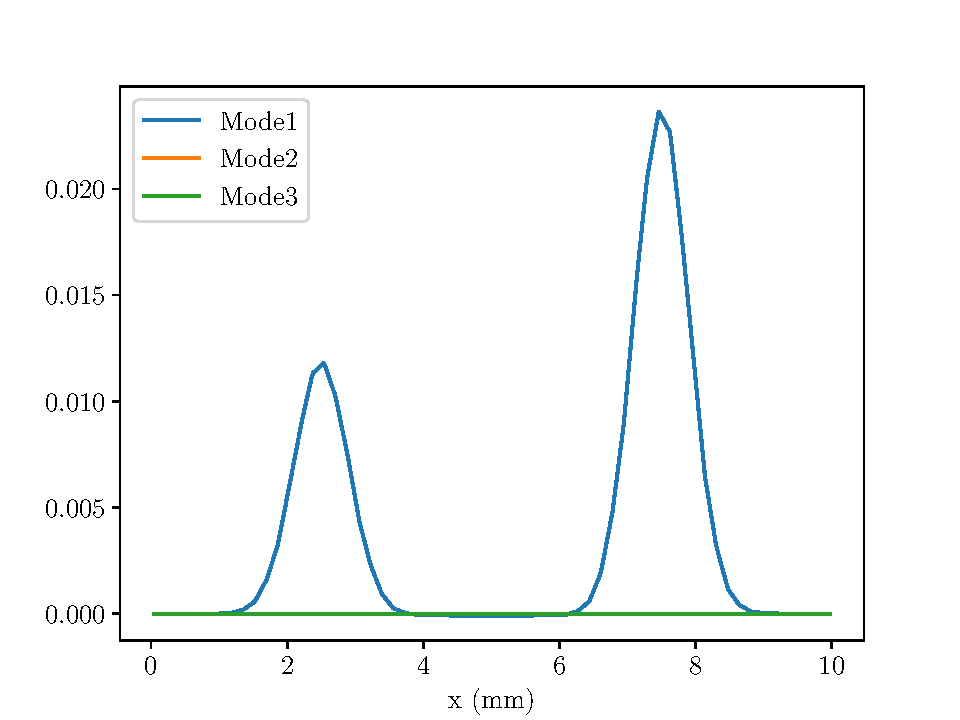
\includegraphics[width=\linewidth]{Figures/Trained_Space_modes3.pdf}
        \caption{Trained space modes}
    \end{subfigure}
    \caption{Modes initialisation (from 1 mode \& $n_p=10$ to $3$ modes \& $n_p=50$.}
    \label{fig:InitialisationModes_Coarse}
\end{figure}

\subsection{Link with literature}

\cite{giacoma_toward_2015} showed that using a coarser mesh to initialised the reduced-order basis can drastically decrease the number of required iterations to build a reduced-order model. Using the NN-PGD based on the hiDeNN framework, this idea can easily be used in the training strategy to start with coarser mesh and transfer the computed mesh onto the more refined mesh later in the training.